\documentclass[11pt]{article}\usepackage[]{graphicx}\usepackage[]{color}
%% maxwidth is the original width if it is less than linewidth
%% otherwise use linewidth (to make sure the graphics do not exceed the margin)
\makeatletter
\def\maxwidth{ %
  \ifdim\Gin@nat@width>\linewidth
    \linewidth
  \else
    \Gin@nat@width
  \fi
}
\makeatother

\definecolor{fgcolor}{rgb}{0.345, 0.345, 0.345}
\newcommand{\hlnum}[1]{\textcolor[rgb]{0.686,0.059,0.569}{#1}}%
\newcommand{\hlstr}[1]{\textcolor[rgb]{0.192,0.494,0.8}{#1}}%
\newcommand{\hlcom}[1]{\textcolor[rgb]{0.678,0.584,0.686}{\textit{#1}}}%
\newcommand{\hlopt}[1]{\textcolor[rgb]{0,0,0}{#1}}%
\newcommand{\hlstd}[1]{\textcolor[rgb]{0.345,0.345,0.345}{#1}}%
\newcommand{\hlkwa}[1]{\textcolor[rgb]{0.161,0.373,0.58}{\textbf{#1}}}%
\newcommand{\hlkwb}[1]{\textcolor[rgb]{0.69,0.353,0.396}{#1}}%
\newcommand{\hlkwc}[1]{\textcolor[rgb]{0.333,0.667,0.333}{#1}}%
\newcommand{\hlkwd}[1]{\textcolor[rgb]{0.737,0.353,0.396}{\textbf{#1}}}%

\usepackage{framed}
\makeatletter
\newenvironment{kframe}{%
 \def\at@end@of@kframe{}%
 \ifinner\ifhmode%
  \def\at@end@of@kframe{\end{minipage}}%
  \begin{minipage}{\columnwidth}%
 \fi\fi%
 \def\FrameCommand##1{\hskip\@totalleftmargin \hskip-\fboxsep
 \colorbox{shadecolor}{##1}\hskip-\fboxsep
     % There is no \\@totalrightmargin, so:
     \hskip-\linewidth \hskip-\@totalleftmargin \hskip\columnwidth}%
 \MakeFramed {\advance\hsize-\width
   \@totalleftmargin\z@ \linewidth\hsize
   \@setminipage}}%
 {\par\unskip\endMakeFramed%
 \at@end@of@kframe}
\makeatother

\definecolor{shadecolor}{rgb}{.97, .97, .97}
\definecolor{messagecolor}{rgb}{0, 0, 0}
\definecolor{warningcolor}{rgb}{1, 0, 1}
\definecolor{errorcolor}{rgb}{1, 0, 0}
\newenvironment{knitrout}{}{} % an empty environment to be redefined in TeX

\usepackage{alltt}

\usepackage{hyperref, lastpage, fancyhdr,multicol,caption,subcaption,tabularx}
\usepackage{amsmath,graphicx}
\usepackage{float}

\usepackage{geometry}
\usepackage{pdflscape}



\topmargin      -1.5cm   % read Lamport p.163
\oddsidemargin  -0.04cm  % read Lamport p.163
\evensidemargin -0.04cm  % same as oddsidemargin but for left-hand pages
\textwidth      16.59cm
\textheight     23.94cm
\parskip         7.2pt   % sets spacing between paragraphs
\parindent         0pt   % sets leading space for paragraphs
\pagestyle{empty}        % Uncomment if don't want page numbers
\pagestyle{fancyplain}

\usepackage{natbib} %need this for bibtex
\IfFileExists{upquote.sty}{\usepackage{upquote}}{}

\lhead{}
\chead{}
\rhead{}

\usepackage{setspace} %for double spacing
\doublespacing
\IfFileExists{upquote.sty}{\usepackage{upquote}}{}
\begin{document}




\begin{knitrout}
\definecolor{shadecolor}{rgb}{0.969, 0.969, 0.969}\color{fgcolor}
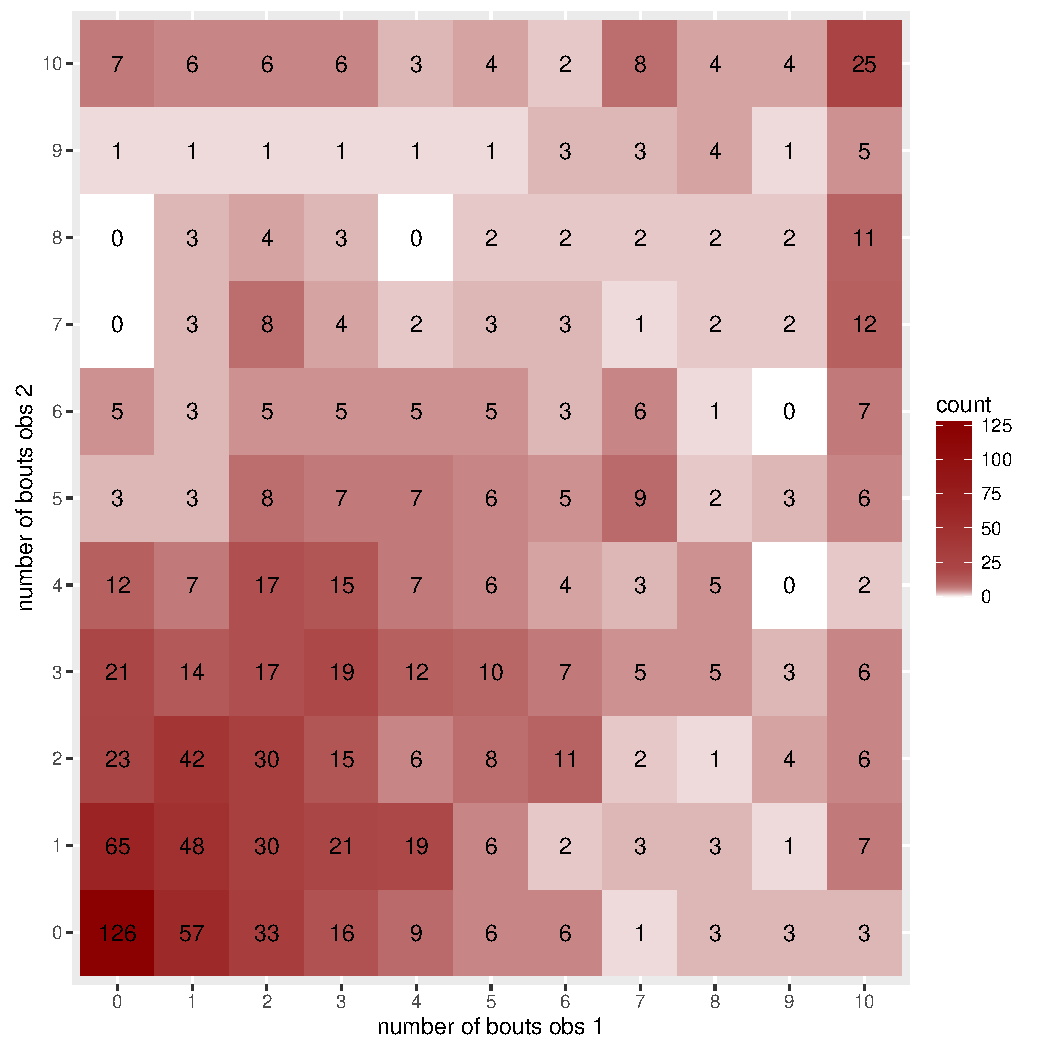
\includegraphics[width=\maxwidth]{figure/p1-1} 

\end{knitrout}

\begin{knitrout}
\definecolor{shadecolor}{rgb}{0.969, 0.969, 0.969}\color{fgcolor}
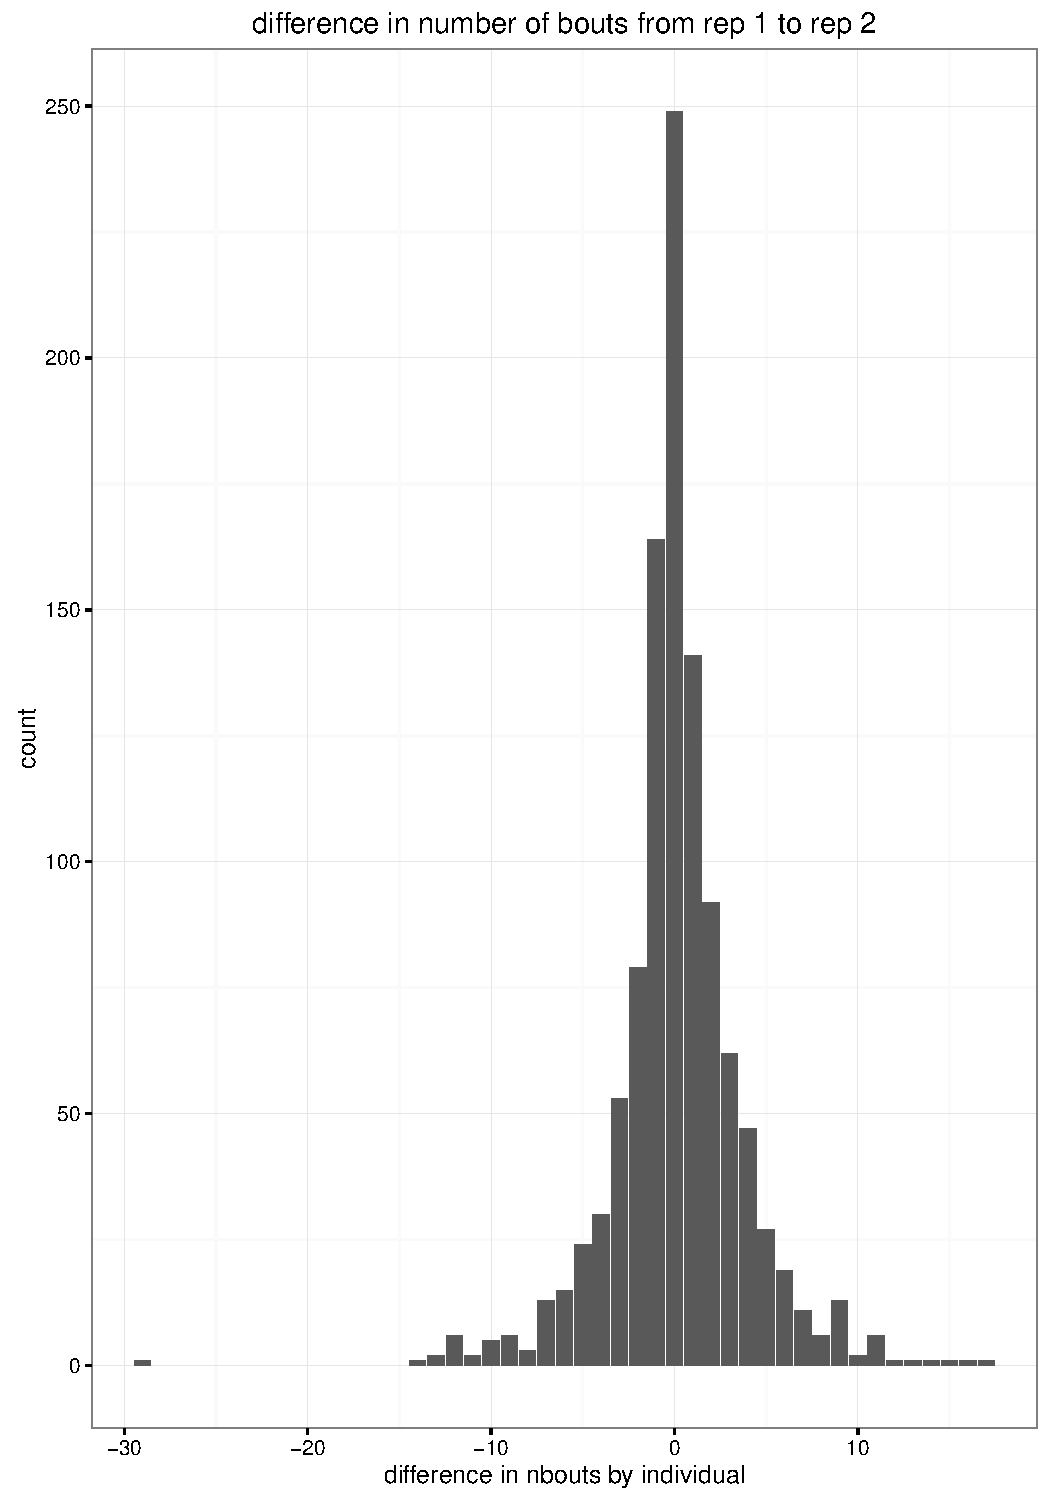
\includegraphics[width=\maxwidth]{figure/p1a-1} 

\end{knitrout}

\begin{knitrout}
\definecolor{shadecolor}{rgb}{0.969, 0.969, 0.969}\color{fgcolor}
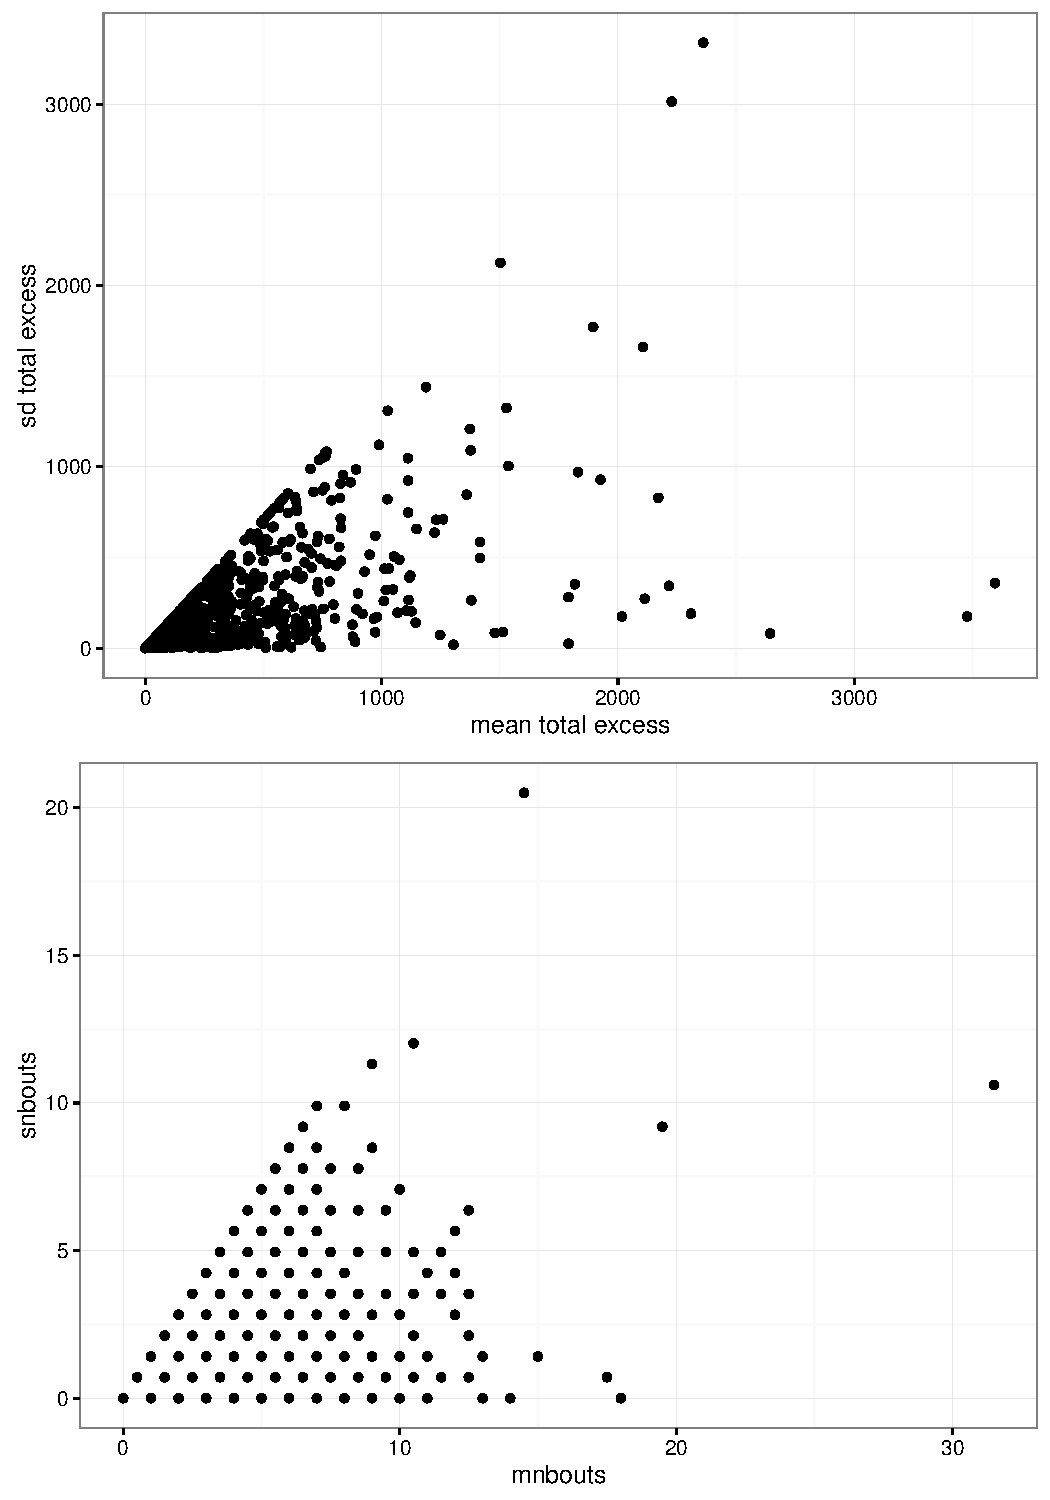
\includegraphics[width=\maxwidth]{figure/p1b-1} 

\end{knitrout}




\begin{knitrout}
\definecolor{shadecolor}{rgb}{0.969, 0.969, 0.969}\color{fgcolor}
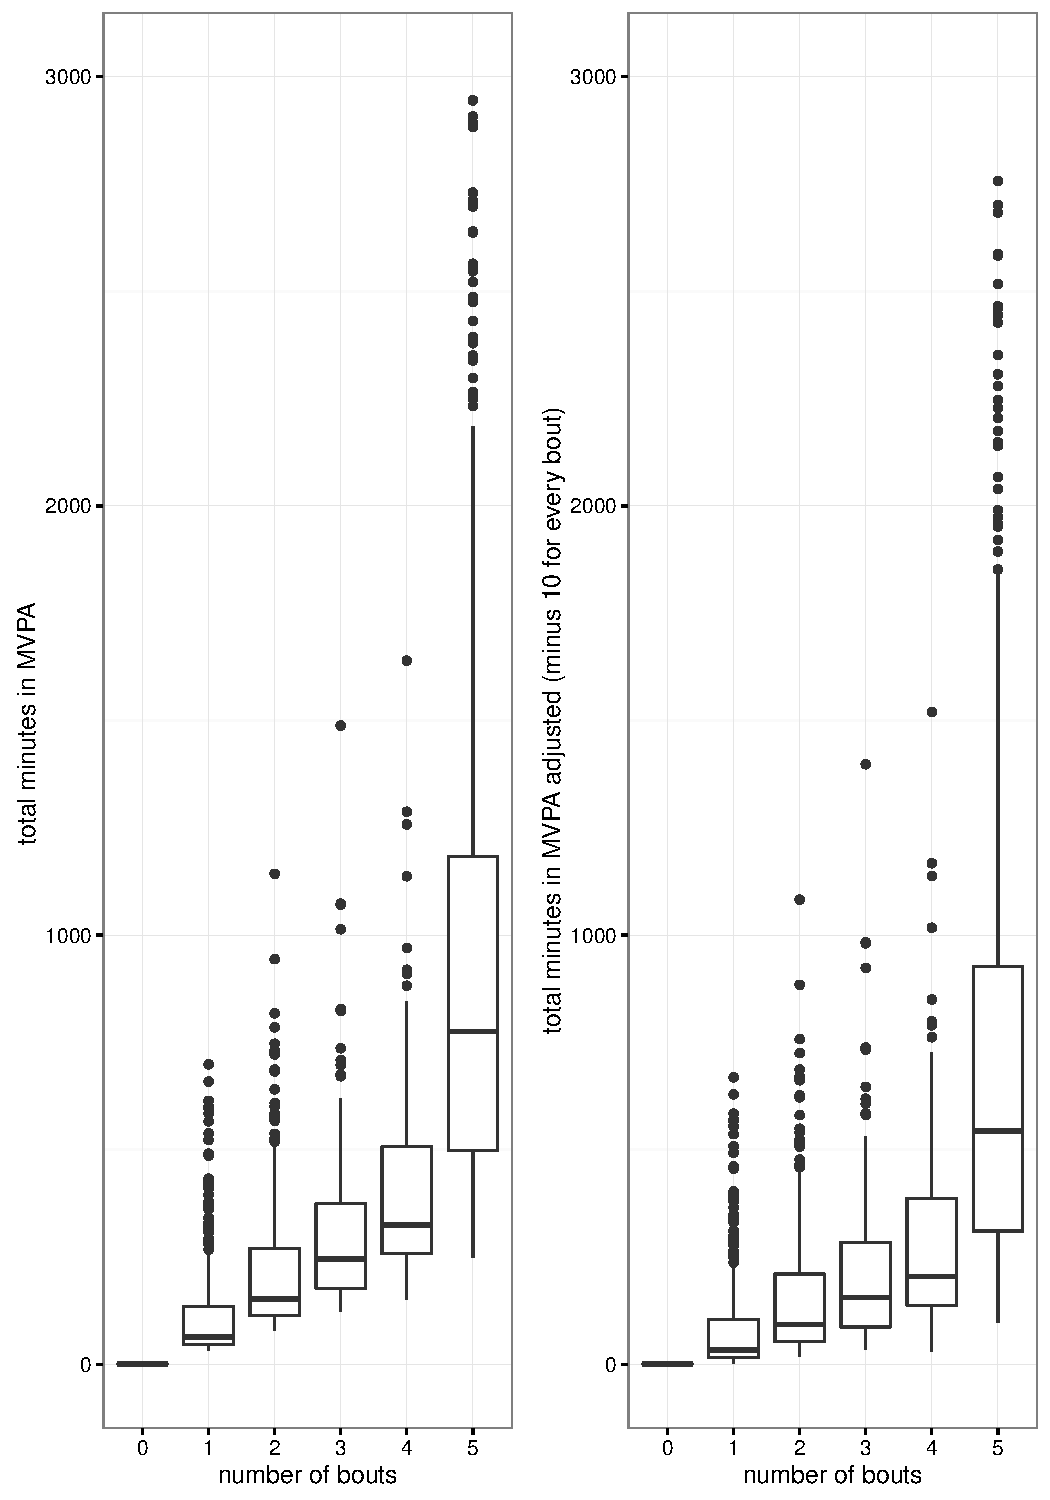
\includegraphics[width=\maxwidth]{figure/p2-1} 

\end{knitrout}

\begin{knitrout}
\definecolor{shadecolor}{rgb}{0.969, 0.969, 0.969}\color{fgcolor}
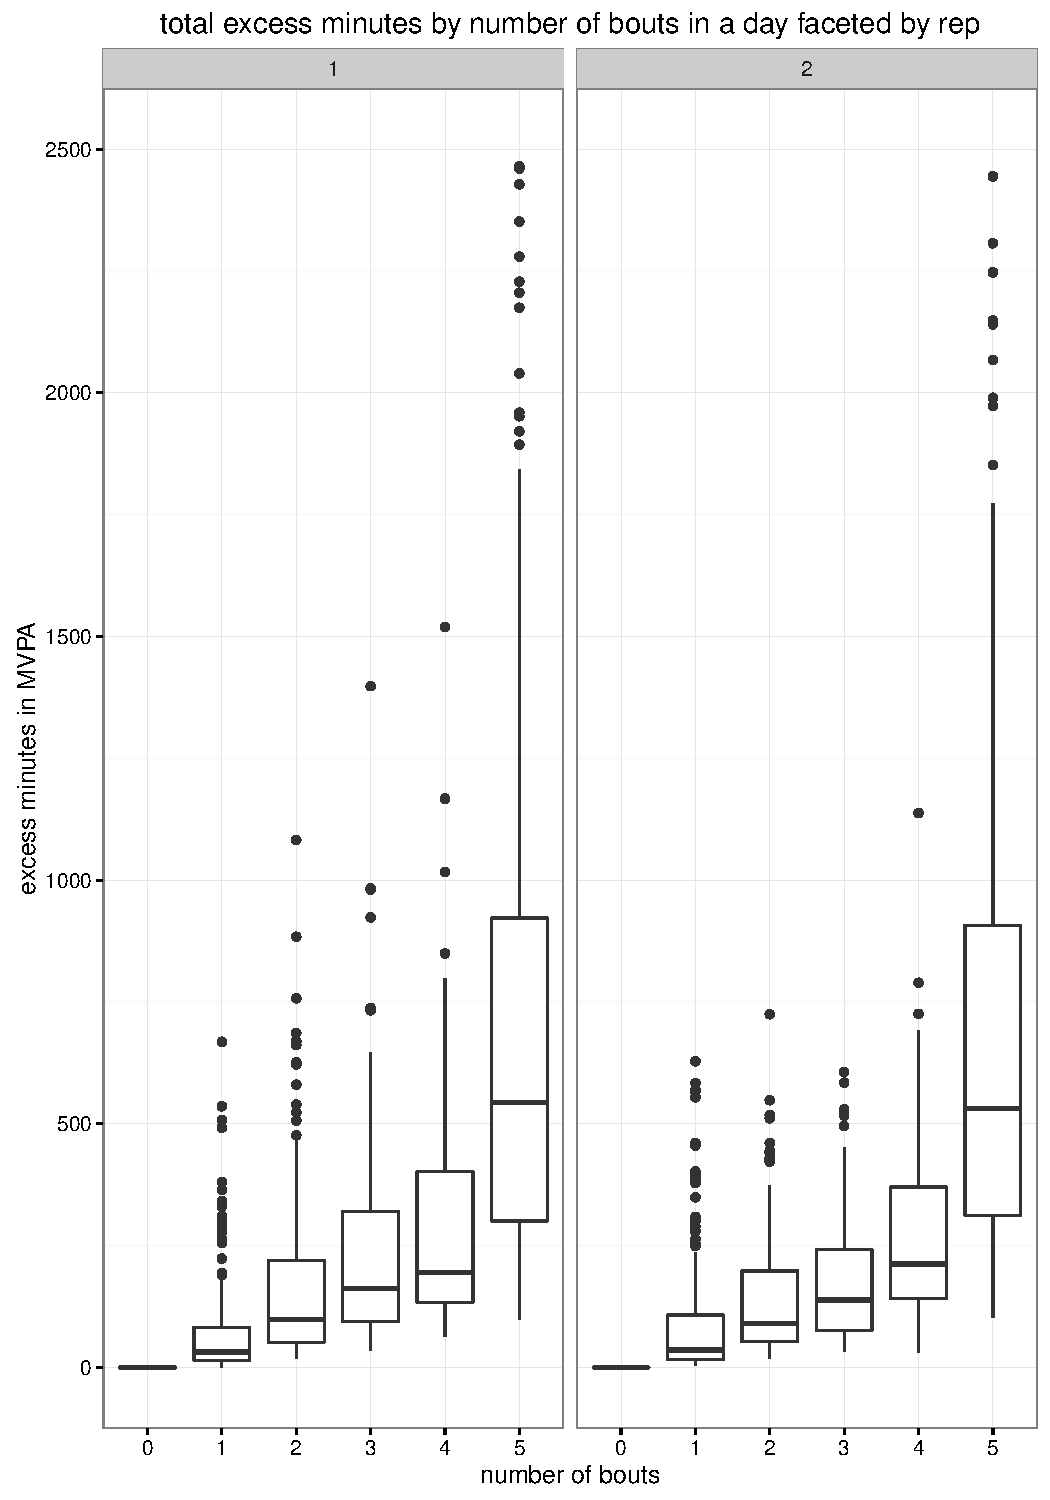
\includegraphics[width=\maxwidth]{figure/p2bb-1} 

\end{knitrout}

\begin{knitrout}
\definecolor{shadecolor}{rgb}{0.969, 0.969, 0.969}\color{fgcolor}
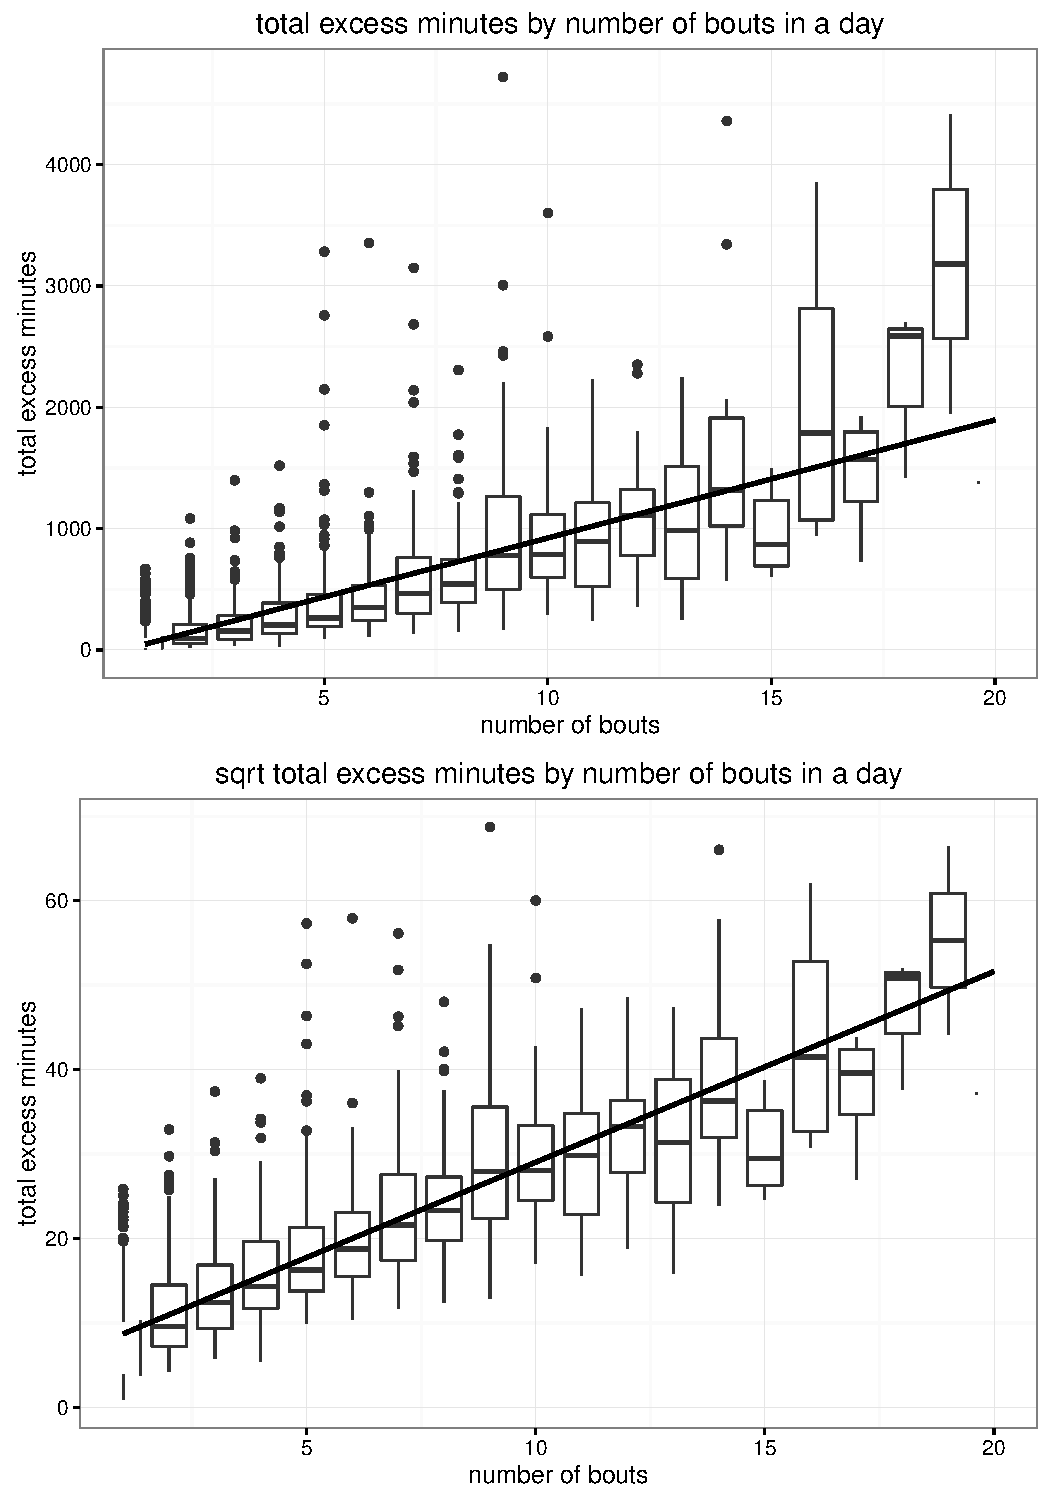
\includegraphics[width=\maxwidth]{figure/p3-1} 

\end{knitrout}


\begin{knitrout}
\definecolor{shadecolor}{rgb}{0.969, 0.969, 0.969}\color{fgcolor}
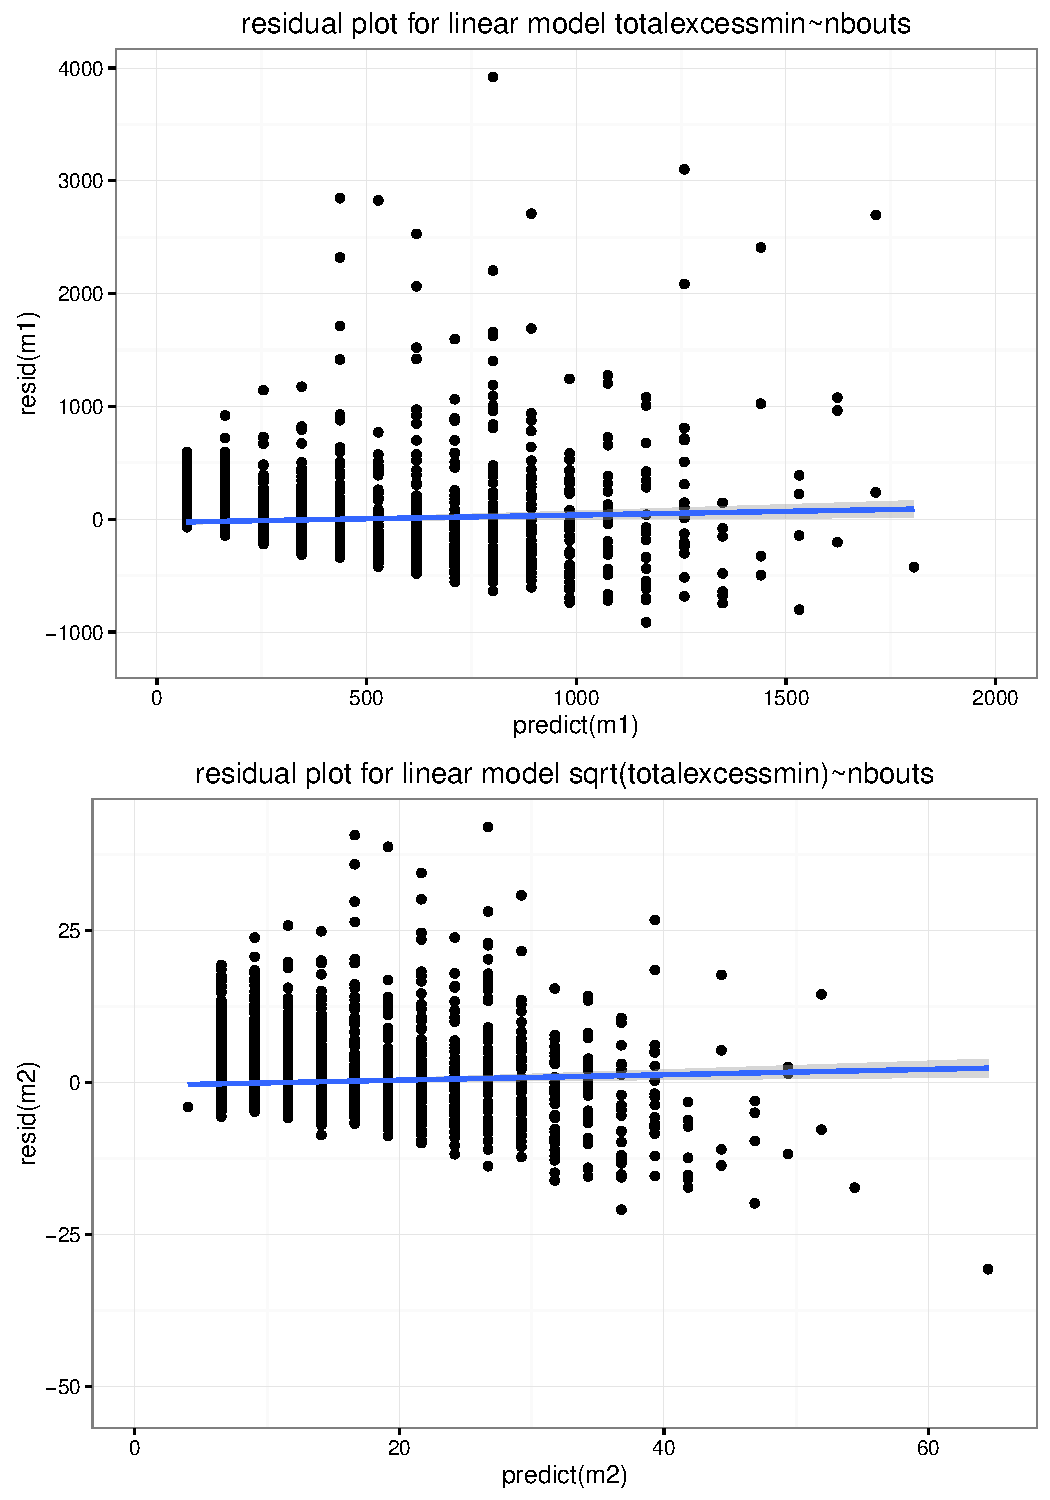
\includegraphics[width=\maxwidth]{figure/resid-1} 

\end{knitrout}



\begin{knitrout}
\definecolor{shadecolor}{rgb}{0.969, 0.969, 0.969}\color{fgcolor}
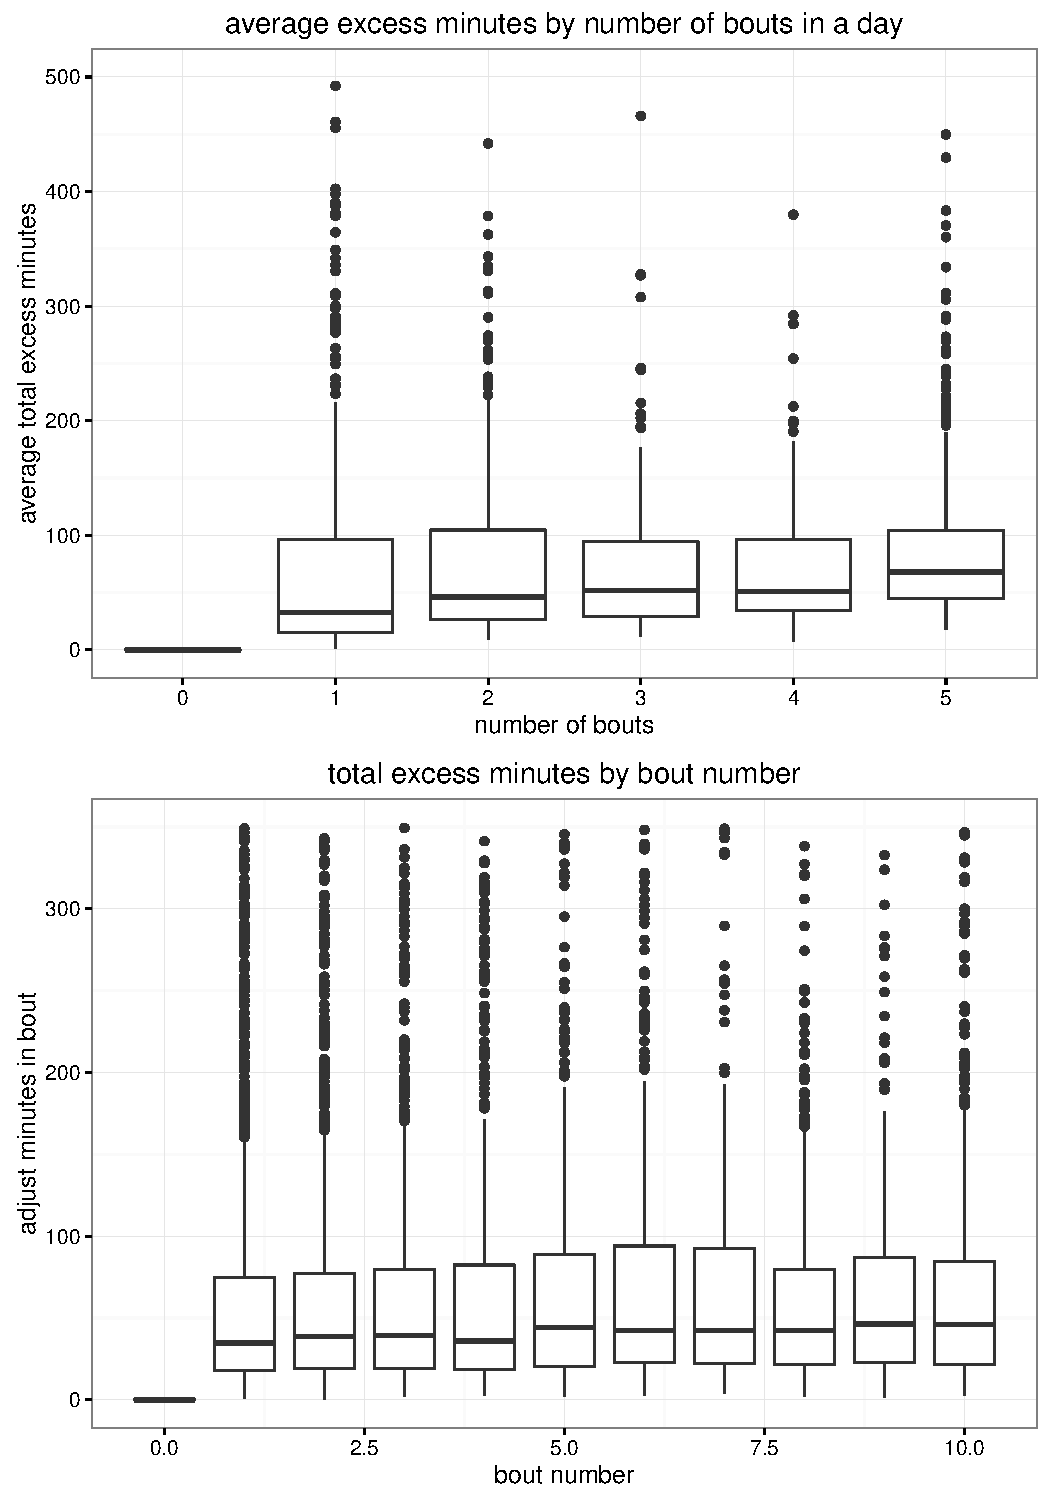
\includegraphics[width=\maxwidth]{figure/p2b-1} 

\end{knitrout}


\begin{knitrout}
\definecolor{shadecolor}{rgb}{0.969, 0.969, 0.969}\color{fgcolor}
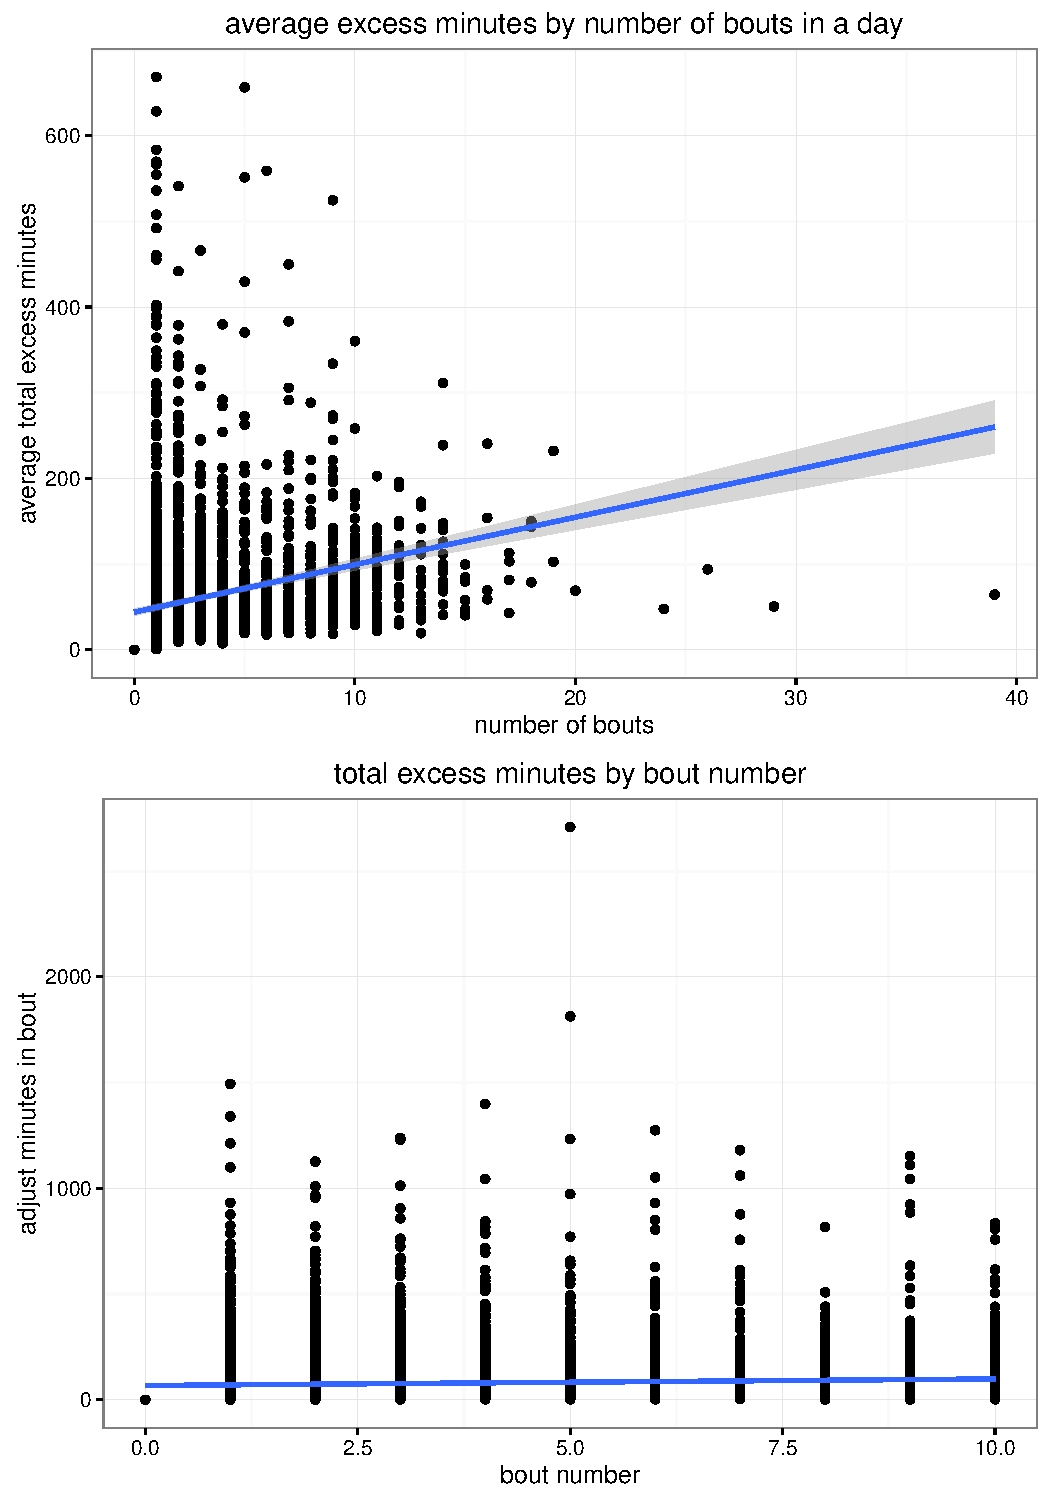
\includegraphics[width=\maxwidth]{figure/p2c-1} 

\end{knitrout}




\begin{knitrout}
\definecolor{shadecolor}{rgb}{0.969, 0.969, 0.969}\color{fgcolor}
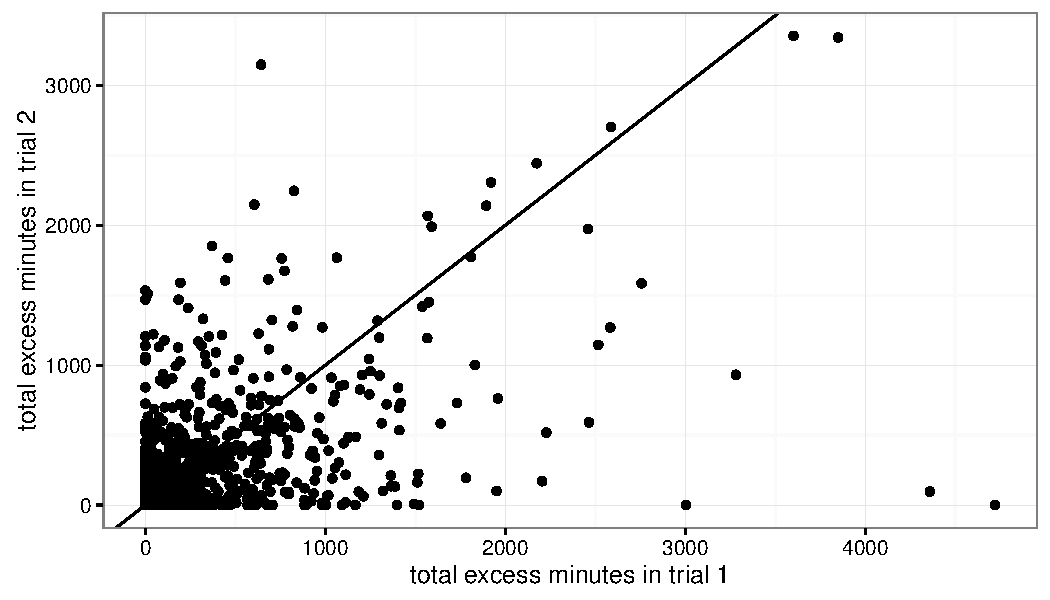
\includegraphics[width=\maxwidth]{figure/p4-1} 

\end{knitrout}



\begin{knitrout}
\definecolor{shadecolor}{rgb}{0.969, 0.969, 0.969}\color{fgcolor}
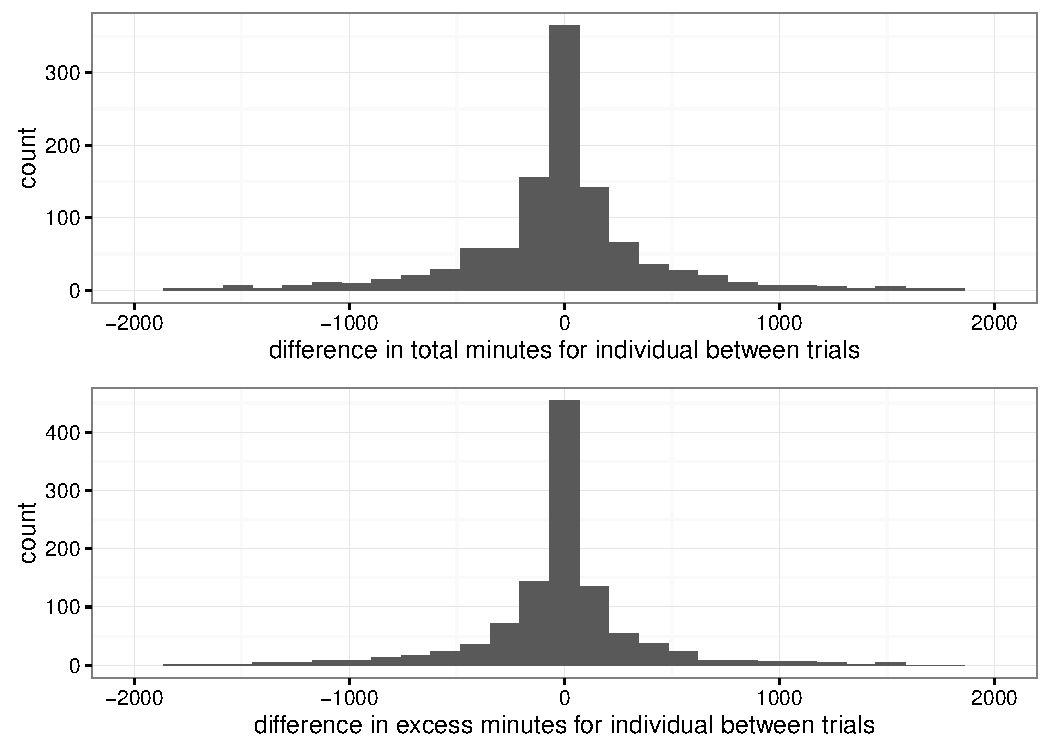
\includegraphics[width=\maxwidth]{figure/p5-1} 

\end{knitrout}


\begin{knitrout}
\definecolor{shadecolor}{rgb}{0.969, 0.969, 0.969}\color{fgcolor}
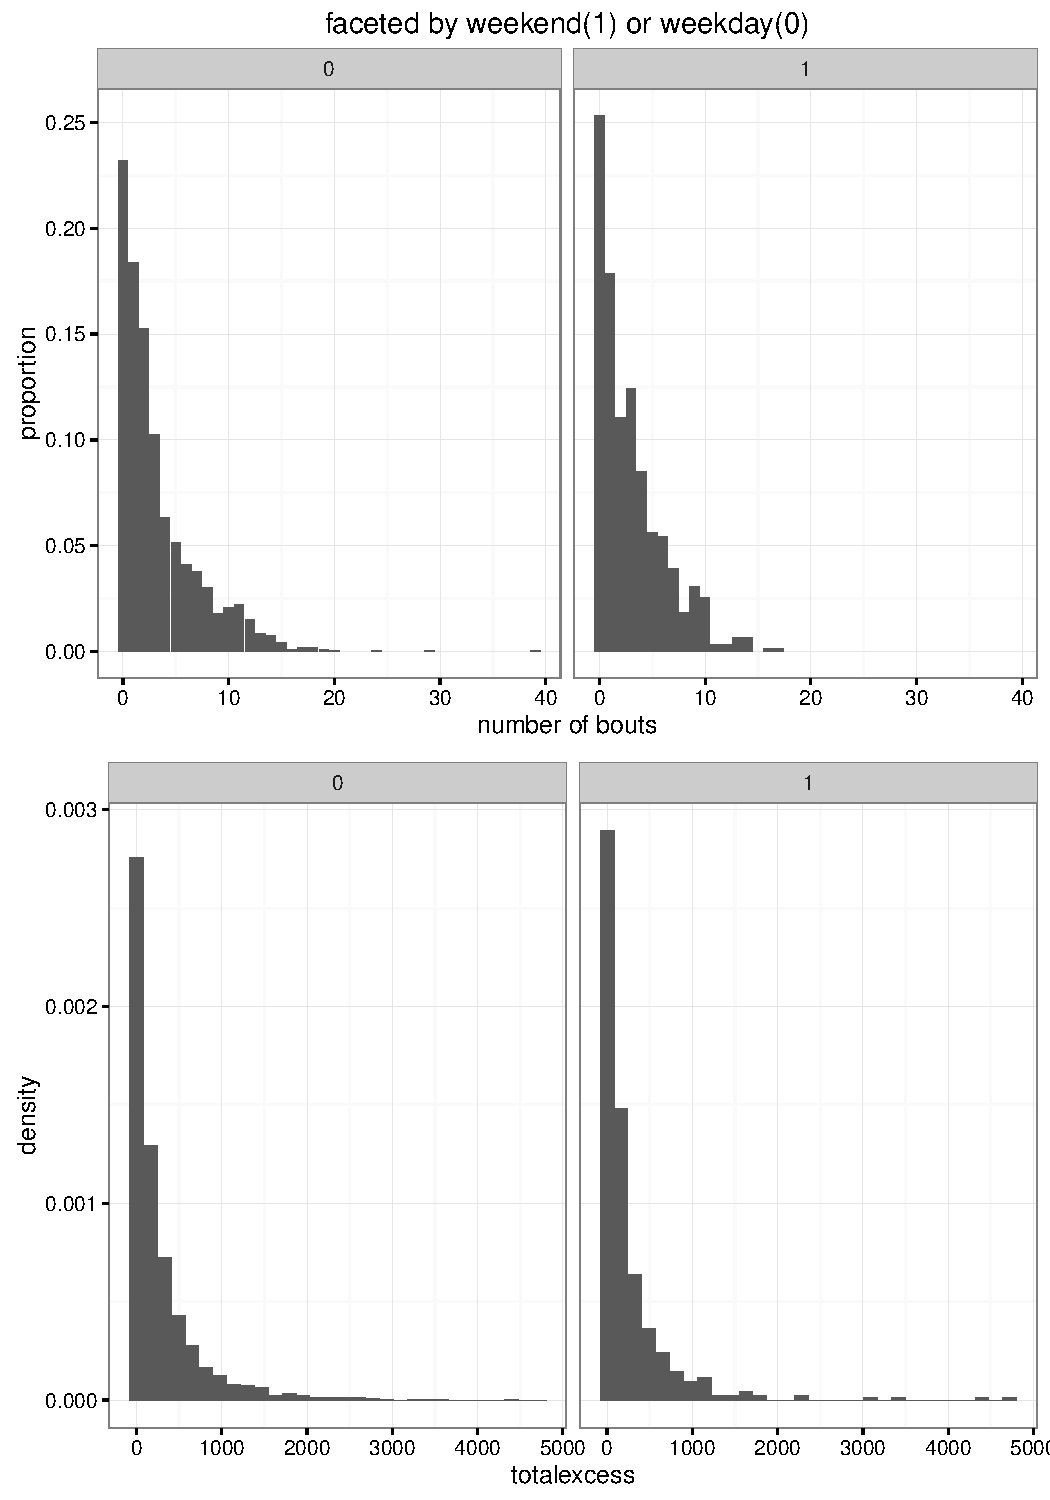
\includegraphics[width=\maxwidth]{figure/p6-1} 

\end{knitrout}


\begin{knitrout}
\definecolor{shadecolor}{rgb}{0.969, 0.969, 0.969}\color{fgcolor}
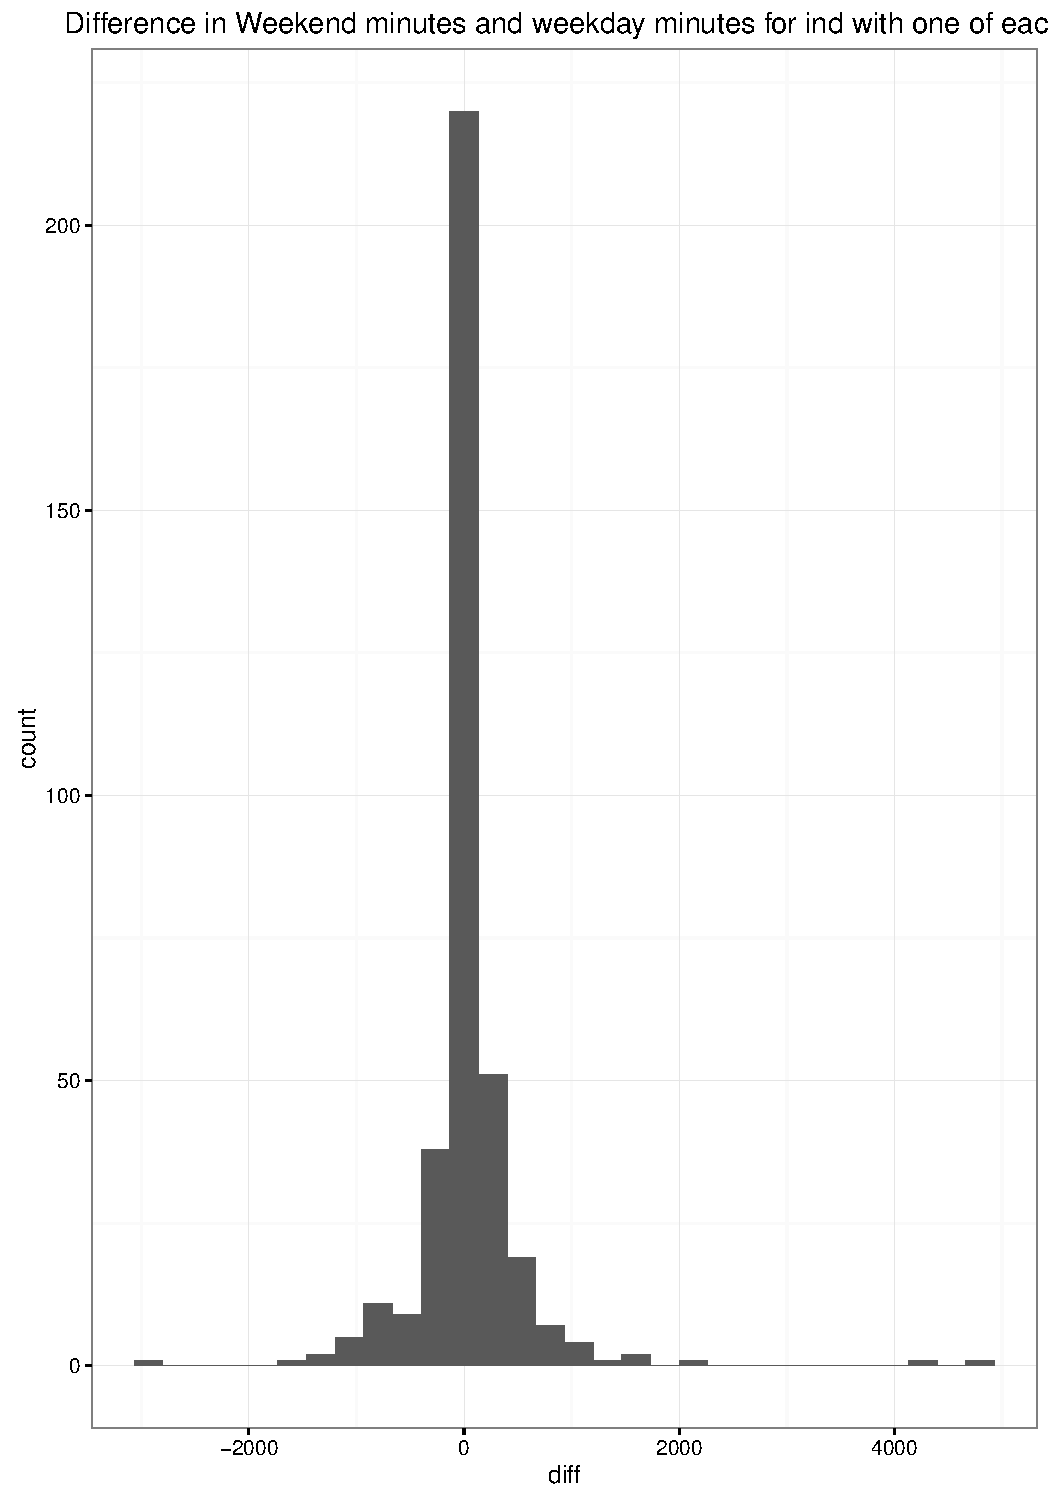
\includegraphics[width=\maxwidth]{figure/p7-1} 

\end{knitrout}

%-------------------------------------
%tests



\begin{knitrout}
\definecolor{shadecolor}{rgb}{0.969, 0.969, 0.969}\color{fgcolor}\begin{kframe}
\begin{alltt}
\hlcom{#test difference in mean totalexcess min from trial 1 to trial 2 paired by individual}
\hlstd{trial1} \hlkwb{<-} \hlstd{bouts} \hlopt \hlkwd{group_by}\hlstd{(id)} \hlopt \hlkwd{filter}\hlstd{(}\hlkwd{length}\hlstd{((id))}\hlopt{==}\hlnum{2}\hlstd{, rep}\hlopt{==}\hlnum{1}\hlstd{)}
\hlstd{trial2} \hlkwb{<-} \hlstd{bouts} \hlopt \hlkwd{group_by}\hlstd{(id)} \hlopt \hlkwd{filter}\hlstd{(}\hlkwd{length}\hlstd{((id))}\hlopt{==}\hlnum{2}\hlstd{, rep}\hlopt{==}\hlnum{2}\hlstd{)}

\hlkwd{wilcox.test}\hlstd{(trial1}\hlopt{$}\hlstd{totalexcess,trial2}\hlopt{$}\hlstd{totalexcess,}\hlkwc{paired}\hlstd{=}\hlnum{TRUE}\hlstd{)}
\end{alltt}
\begin{verbatim}
## 
## 	Wilcoxon signed rank test with continuity correction
## 
## data:  trial1$totalexcess and trial2$totalexcess
## V = 245710, p-value = 0.07001
## alternative hypothesis: true location shift is not equal to 0
\end{verbatim}
\end{kframe}
\end{knitrout}

\begin{knitrout}
\definecolor{shadecolor}{rgb}{0.969, 0.969, 0.969}\color{fgcolor}\begin{kframe}
\begin{alltt}
\hlcom{#test difference in distribution of totalexcess min from trial 1 to trial 2}
\hlkwd{ks.test}\hlstd{(bouts}\hlopt{$}\hlstd{totalexcess[bouts}\hlopt{$}\hlstd{rep}\hlopt{==}\hlnum{1}\hlstd{],bouts}\hlopt{$}\hlstd{totalexcess[bouts}\hlopt{$}\hlstd{rep}\hlopt{==}\hlnum{2}\hlstd{])}
\end{alltt}
\begin{verbatim}
## 
## 	Two-sample Kolmogorov-Smirnov test
## 
## data:  bouts$totalexcess[bouts$rep == 1] and bouts$totalexcess[bouts$rep == 2]
## D = 0.034009, p-value = 0.5031
## alternative hypothesis: two-sided
\end{verbatim}
\end{kframe}
\end{knitrout}


\begin{knitrout}
\definecolor{shadecolor}{rgb}{0.969, 0.969, 0.969}\color{fgcolor}\begin{kframe}
\begin{alltt}
\hlcom{#test difference in distribution of  differenced totalexcess min from trial 1 to trial 2 compared to  differenced totalexcess min from trial 2 to trial 1}
\hlstd{a1} \hlkwb{<-} \hlstd{(trial2}\hlopt{$}\hlstd{totalexcess}\hlopt{-}\hlstd{trial1}\hlopt{$}\hlstd{totalexcess)}
\hlstd{a2} \hlkwb{<-} \hlstd{(trial1}\hlopt{$}\hlstd{totalexcess}\hlopt{-}\hlstd{trial2}\hlopt{$}\hlstd{totalexcess)}
\hlkwd{ks.test}\hlstd{(a1,a2)}
\end{alltt}
\begin{verbatim}
## 
## 	Two-sample Kolmogorov-Smirnov test
## 
## data:  a1 and a2
## D = 0.04977, p-value = 0.1361
## alternative hypothesis: two-sided
\end{verbatim}
\end{kframe}
\end{knitrout}



\begin{knitrout}
\definecolor{shadecolor}{rgb}{0.969, 0.969, 0.969}\color{fgcolor}\begin{kframe}
\begin{alltt}
\hlcom{#difference in mean nbouts min from trial 1 to trial 2}
\hlkwd{wilcox.test}\hlstd{(trial1}\hlopt{$}\hlstd{nbouts,trial2}\hlopt{$}\hlstd{nbouts,}\hlkwc{paired}\hlstd{=}\hlnum{TRUE}\hlstd{)}
\end{alltt}
\begin{verbatim}
## 
## 	Wilcoxon signed rank test with continuity correction
## 
## data:  trial1$nbouts and trial2$nbouts
## V = 187960, p-value = 0.06021
## alternative hypothesis: true location shift is not equal to 0
\end{verbatim}
\end{kframe}
\end{knitrout}


\begin{knitrout}
\definecolor{shadecolor}{rgb}{0.969, 0.969, 0.969}\color{fgcolor}\begin{kframe}
\begin{alltt}
\hlcom{#test marginal distributional differences in nbouts from trial 1 to trial 2}
\hlkwd{ks.test}\hlstd{(bouts}\hlopt{$}\hlstd{nbouts[bouts}\hlopt{$}\hlstd{rep}\hlopt{==}\hlnum{1}\hlstd{],bouts}\hlopt{$}\hlstd{nbouts[bouts}\hlopt{$}\hlstd{rep}\hlopt{==}\hlnum{2}\hlstd{])}
\end{alltt}
\begin{verbatim}
## 
## 	Two-sample Kolmogorov-Smirnov test
## 
## data:  bouts$nbouts[bouts$rep == 1] and bouts$nbouts[bouts$rep == 2]
## D = 0.024617, p-value = 0.8674
## alternative hypothesis: two-sided
\end{verbatim}
\end{kframe}
\end{knitrout}

\begin{knitrout}
\definecolor{shadecolor}{rgb}{0.969, 0.969, 0.969}\color{fgcolor}\begin{kframe}
\begin{alltt}
\hlcom{#nbouts of weekday vs weekend}
\hlkwd{ks.test}\hlstd{(bouts}\hlopt{$}\hlstd{nbouts[bouts}\hlopt{$}\hlstd{Weekend}\hlopt{==}\hlnum{0}\hlstd{],bouts}\hlopt{$}\hlstd{nbouts[bouts}\hlopt{$}\hlstd{Weekend}\hlopt{==}\hlnum{1}\hlstd{])}
\end{alltt}
\begin{verbatim}
## 
## 	Two-sample Kolmogorov-Smirnov test
## 
## data:  bouts$nbouts[bouts$Weekend == 0] and bouts$nbouts[bouts$Weekend == 1]
## D = 0.042311, p-value = 0.4138
## alternative hypothesis: two-sided
\end{verbatim}
\begin{alltt}
\hlcom{#excess minutes of weekday vs weekend}
\hlkwd{ks.test}\hlstd{(bouts}\hlopt{$}\hlstd{totalexcess[bouts}\hlopt{$}\hlstd{Weekend}\hlopt{==}\hlnum{0}\hlstd{],bouts}\hlopt{$}\hlstd{totalexcess[bouts}\hlopt{$}\hlstd{Weekend}\hlopt{==}\hlnum{1}\hlstd{])}
\end{alltt}
\begin{verbatim}
## 
## 	Two-sample Kolmogorov-Smirnov test
## 
## data:  bouts$totalexcess[bouts$Weekend == 0] and bouts$totalexcess[bouts$Weekend == 1]
## D = 0.062531, p-value = 0.06534
## alternative hypothesis: two-sided
\end{verbatim}
\end{kframe}
\end{knitrout}

\begin{knitrout}
\definecolor{shadecolor}{rgb}{0.969, 0.969, 0.969}\color{fgcolor}\begin{kframe}
\begin{alltt}
\hlcom{#test difference in means of total excess in weekday vs weekend for those with both}
\hlstd{week1weekend1} \hlkwb{<-} \hlstd{bouts} \hlopt \hlkwd{group_by}\hlstd{(id)} \hlopt \hlkwd{filter}\hlstd{(}\hlkwd{length}\hlstd{((id))}\hlopt{==}\hlnum{2}\hlstd{,} \hlkwd{sum}\hlstd{(Weekend)}\hlopt{==}\hlnum{1}\hlstd{, rep}\hlopt{==}\hlnum{1}\hlstd{)}
\hlstd{week1weekend2} \hlkwb{<-} \hlstd{bouts} \hlopt \hlkwd{group_by}\hlstd{(id)} \hlopt \hlkwd{filter}\hlstd{(}\hlkwd{length}\hlstd{((id))}\hlopt{==}\hlnum{2}\hlstd{,} \hlkwd{sum}\hlstd{(Weekend)}\hlopt{==}\hlnum{1}\hlstd{, rep}\hlopt{==}\hlnum{2}\hlstd{)}

\hlkwd{wilcox.test}\hlstd{(week1weekend1}\hlopt{$}\hlstd{totalexcess,week1weekend2}\hlopt{$}\hlstd{totalexcess,}\hlkwc{paired}\hlstd{=}\hlnum{TRUE}\hlstd{)}
\end{alltt}
\begin{verbatim}
## 
## 	Wilcoxon signed rank test with continuity correction
## 
## data:  week1weekend1$totalexcess and week1weekend2$totalexcess
## V = 30118, p-value = 0.3099
## alternative hypothesis: true location shift is not equal to 0
\end{verbatim}
\begin{alltt}
\hlcom{#test difference in means of nbouts in weekday vs weekend for those with both}
\hlkwd{wilcox.test}\hlstd{(week1weekend1}\hlopt{$}\hlstd{nbouts,week1weekend2}\hlopt{$}\hlstd{nbouts,}\hlkwc{paired}\hlstd{=}\hlnum{TRUE}\hlstd{)}
\end{alltt}
\begin{verbatim}
## 
## 	Wilcoxon signed rank test with continuity correction
## 
## data:  week1weekend1$nbouts and week1weekend2$nbouts
## V = 22398, p-value = 0.3595
## alternative hypothesis: true location shift is not equal to 0
\end{verbatim}
\end{kframe}
\end{knitrout}


\begin{knitrout}
\definecolor{shadecolor}{rgb}{0.969, 0.969, 0.969}\color{fgcolor}\begin{kframe}
\begin{alltt}
\hlcom{#test for difference in avg total excess mins by number of bouts}
\hlcom{#nonparametric test since normality doesn't hold}
\hlkwd{kruskal.test}\hlstd{(avgtotalexcess}\hlopt{~}\hlstd{nbouts,}\hlkwc{data}\hlstd{=}\hlkwd{subset}\hlstd{(bouts,nbouts}\hlopt{>}\hlnum{0}\hlstd{))}
\end{alltt}
\begin{verbatim}
## 
## 	Kruskal-Wallis rank sum test
## 
## data:  avgtotalexcess by nbouts
## Kruskal-Wallis chi-squared = 136.9, df = 23, p-value < 2.2e-16
\end{verbatim}
\begin{alltt}
\hlkwd{kruskal.test}\hlstd{(avgtotalexcess}\hlopt{~}\hlstd{nbouts,}\hlkwc{data}\hlstd{=}\hlkwd{subset}\hlstd{(bouts,nbouts}\hlopt{>}\hlnum{0}\hlopt{&}\hlstd{nbouts}\hlopt{<}\hlnum{11}\hlstd{))}
\end{alltt}
\begin{verbatim}
## 
## 	Kruskal-Wallis rank sum test
## 
## data:  avgtotalexcess by nbouts
## Kruskal-Wallis chi-squared = 101.37, df = 9, p-value < 2.2e-16
\end{verbatim}
\end{kframe}
\end{knitrout}

\begin{knitrout}
\definecolor{shadecolor}{rgb}{0.969, 0.969, 0.969}\color{fgcolor}\begin{kframe}
\begin{alltt}
\hlcom{#linear trend on  avgtotalexcess minutes with nbouts as covariate}
\hlstd{m1lm} \hlkwb{<-} \hlkwd{lm}\hlstd{((avgtotalexcess)}\hlopt{~}\hlstd{(nbouts),}\hlkwc{data}\hlstd{=}\hlkwd{subset}\hlstd{(bouts,nbouts}\hlopt{>}\hlnum{0}\hlstd{))}
\hlkwd{summary}\hlstd{(m1lm)}
\end{alltt}
\begin{verbatim}
## 
## Call:
## lm(formula = (avgtotalexcess) ~ (nbouts), data = subset(bouts, 
##     nbouts > 0))
## 
## Residuals:
##    Min     1Q Median     3Q    Max 
## -76.60 -50.48 -27.62  20.02 591.14 
## 
## Coefficients:
##             Estimate Std. Error t value Pr(>|t|)    
## (Intercept)  76.2126     2.9927  25.466   <2e-16 ***
## nbouts        1.1982     0.5323   2.251   0.0245 *  
## ---
## Signif. codes:  0 '***' 0.001 '**' 0.01 '*' 0.05 '.' 0.1 ' ' 1
## 
## Residual standard error: 83.13 on 1808 degrees of freedom
## Multiple R-squared:  0.002795,	Adjusted R-squared:  0.002243 
## F-statistic: 5.067 on 1 and 1808 DF,  p-value: 0.02451
\end{verbatim}
\begin{alltt}
\hlstd{m1lmb} \hlkwb{<-} \hlkwd{lm}\hlstd{((avgtotalexcess)}\hlopt{~}\hlstd{(nbouts),}\hlkwc{data}\hlstd{=}\hlkwd{subset}\hlstd{(bouts,nbouts}\hlopt{>}\hlnum{0}\hlopt{&}\hlstd{nbouts}\hlopt{<}\hlnum{11}\hlstd{))}
\hlkwd{summary}\hlstd{(m1lmb)}
\end{alltt}
\begin{verbatim}
## 
## Call:
## lm(formula = (avgtotalexcess) ~ (nbouts), data = subset(bouts, 
##     nbouts > 0 & nbouts < 11))
## 
## Residuals:
##    Min     1Q Median     3Q    Max 
## -75.86 -51.23 -29.87  19.85 591.88 
## 
## Coefficients:
##             Estimate Std. Error t value Pr(>|t|)    
## (Intercept)  75.1162     3.5804  20.980   <2e-16 ***
## nbouts        1.5505     0.8238   1.882     0.06 .  
## ---
## Signif. codes:  0 '***' 0.001 '**' 0.01 '*' 0.05 '.' 0.1 ' ' 1
## 
## Residual standard error: 85.28 on 1675 degrees of freedom
## Multiple R-squared:  0.00211,	Adjusted R-squared:  0.001515 
## F-statistic: 3.542 on 1 and 1675 DF,  p-value: 0.05999
\end{verbatim}
\end{kframe}
\end{knitrout}



\begin{knitrout}
\definecolor{shadecolor}{rgb}{0.969, 0.969, 0.969}\color{fgcolor}\begin{kframe}
\begin{alltt}
\hlcom{#test for diff in total excess mins by bout number}
\hlcom{#nonparametric test since normality doesn't hold}
\hlkwd{kruskal.test}\hlstd{(totalpadj}\hlopt{~}\hlstd{bout,}\hlkwc{data}\hlstd{=}\hlkwd{subset}\hlstd{(bybout,bout}\hlopt{>}\hlnum{0}\hlstd{))}
\end{alltt}
\begin{verbatim}
## 
## 	Kruskal-Wallis rank sum test
## 
## data:  totalpadj by bout
## Kruskal-Wallis chi-squared = 50.569, df = 38, p-value = 0.08341
\end{verbatim}
\begin{alltt}
\hlkwd{kruskal.test}\hlstd{(totalpadj}\hlopt{~}\hlstd{bout,}\hlkwc{data}\hlstd{=}\hlkwd{subset}\hlstd{(bybout,bout}\hlopt{>}\hlnum{0}\hlopt{&}\hlstd{bout}\hlopt{<}\hlnum{11}\hlstd{))}
\end{alltt}
\begin{verbatim}
## 
## 	Kruskal-Wallis rank sum test
## 
## data:  totalpadj by bout
## Kruskal-Wallis chi-squared = 23.959, df = 9, p-value = 0.004367
\end{verbatim}
\end{kframe}
\end{knitrout}


\begin{knitrout}
\definecolor{shadecolor}{rgb}{0.969, 0.969, 0.969}\color{fgcolor}\begin{kframe}
\begin{alltt}
\hlcom{#linear trend on total excess minutes with bout number as covariate}
\hlstd{m2lm} \hlkwb{<-} \hlkwd{lm}\hlstd{(totalpadj}\hlopt{~}\hlstd{(bout),}\hlkwc{data}\hlstd{=}\hlkwd{subset}\hlstd{(bybout,bout}\hlopt{>}\hlnum{0}\hlstd{))}
\hlkwd{summary}\hlstd{(m2lm)}
\end{alltt}
\begin{verbatim}
## 
## Call:
## lm(formula = totalpadj ~ (bout), data = subset(bybout, bout > 
##     0))
## 
## Residuals:
##     Min      1Q  Median      3Q     Max 
##  -84.41  -64.84  -43.49    7.63 2623.50 
## 
## Coefficients:
##             Estimate Std. Error t value Pr(>|t|)    
## (Intercept)  84.4900     2.2689  37.238   <2e-16 ***
## bout          0.1463     0.4078   0.359     0.72    
## ---
## Signif. codes:  0 '***' 0.001 '**' 0.01 '*' 0.05 '.' 0.1 ' ' 1
## 
## Residual standard error: 130.2 on 7706 degrees of freedom
## Multiple R-squared:  1.671e-05,	Adjusted R-squared:  -0.0001131 
## F-statistic: 0.1287 on 1 and 7706 DF,  p-value: 0.7197
\end{verbatim}
\begin{alltt}
\hlstd{m2lmb} \hlkwb{<-} \hlkwd{lm}\hlstd{(totalpadj}\hlopt{~}\hlstd{(bout),}\hlkwc{data}\hlstd{=}\hlkwd{subset}\hlstd{(bybout,bout}\hlopt{>}\hlnum{0}\hlopt{&}\hlstd{bout}\hlopt{<}\hlnum{11}\hlstd{))}
\hlkwd{summary}\hlstd{(m2lmb)}
\end{alltt}
\begin{verbatim}
## 
## Call:
## lm(formula = totalpadj ~ (bout), data = subset(bybout, bout > 
##     0 & bout < 11))
## 
## Residuals:
##     Min      1Q  Median      3Q     Max 
##  -90.87  -65.00  -43.91    7.54 2621.49 
## 
## Coefficients:
##             Estimate Std. Error t value Pr(>|t|)    
## (Intercept)  80.8104     2.7105  29.814   <2e-16 ***
## bout          1.2850     0.6189   2.076   0.0379 *  
## ---
## Signif. codes:  0 '***' 0.001 '**' 0.01 '*' 0.05 '.' 0.1 ' ' 1
## 
## Residual standard error: 131.7 on 7257 degrees of freedom
## Multiple R-squared:  0.0005938,	Adjusted R-squared:  0.0004561 
## F-statistic: 4.312 on 1 and 7257 DF,  p-value: 0.03789
\end{verbatim}
\end{kframe}
\end{knitrout}


\begin{knitrout}
\definecolor{shadecolor}{rgb}{0.969, 0.969, 0.969}\color{fgcolor}\begin{kframe}
\begin{alltt}
\hlcom{#testing marginal homogeneity of 2 way table of nbouts}
\hlstd{ct1} \hlkwb{<-} \hlkwd{matrix}\hlstd{(}\hlkwd{table}\hlstd{(trial1}\hlopt{$}\hlstd{nbouts,trial2}\hlopt{$}\hlstd{nbouts)[}\hlnum{1}\hlopt{:}\hlnum{10}\hlstd{,}\hlnum{1}\hlopt{:}\hlnum{10}\hlstd{],}\hlkwc{nrow}\hlstd{=}\hlnum{10}\hlstd{,}\hlkwc{byrow}\hlstd{=T)}
\hlkwd{stuart.maxwell.mh}\hlstd{(ct1[}\hlnum{1}\hlopt{:}\hlnum{6}\hlstd{,}\hlnum{1}\hlopt{:}\hlnum{6}\hlstd{])}
\end{alltt}
\begin{verbatim}
##  Stuart-Maxwell marginal homogeneity
## 
##  Subjects = 584 
##    Raters = 2 
##     Chisq = 1.39 
## 
##  Chisq(4) = 1.39 
##   p-value = 0.845
\end{verbatim}
\begin{alltt}
\hlkwd{stuart.maxwell.mh}\hlstd{(ct1)}
\end{alltt}
\begin{verbatim}
##  Stuart-Maxwell marginal homogeneity
## 
##  Subjects = 845 
##    Raters = 2 
##     Chisq = 4.54 
## 
##  Chisq(8) = 4.54 
##   p-value = 0.805
\end{verbatim}
\end{kframe}
\end{knitrout}


\begin{knitrout}
\definecolor{shadecolor}{rgb}{0.969, 0.969, 0.969}\color{fgcolor}\begin{kframe}
\begin{alltt}
\hlcom{#Bowker's test of symmetry, ie. generalization of McNemar's test}
\hlkwd{mcnemar.test}\hlstd{(ct1[}\hlnum{1}\hlopt{:}\hlnum{6}\hlstd{,}\hlnum{1}\hlopt{:}\hlnum{6}\hlstd{])}
\end{alltt}
\begin{verbatim}
## 
## 	McNemar's Chi-squared test
## 
## data:  ct1[1:6, 1:6]
## McNemar's chi-squared = 20.679, df = 15, p-value = 0.1474
\end{verbatim}
\begin{alltt}
\hlkwd{mcnemar.test}\hlstd{(ct1)}
\end{alltt}
\begin{verbatim}
## 
## 	McNemar's Chi-squared test
## 
## data:  ct1
## McNemar's chi-squared = 52.875, df = 45, p-value = 0.1961
\end{verbatim}
\end{kframe}
\end{knitrout}




\begin{knitrout}
\definecolor{shadecolor}{rgb}{0.969, 0.969, 0.969}\color{fgcolor}\begin{kframe}
\begin{alltt}
\hlcom{#permutation test}
\hlcom{#H_0 : sum |lower.tri-upper.tri|  = 0, ie. trial 1 and trial 2 exchangeable}
\hlcom{# H_a : sum > 0, not exchangeable}
\hlstd{obs} \hlkwb{<-} \hlkwd{sum}\hlstd{(}\hlkwd{abs}\hlstd{(ct1[}\hlkwd{lower.tri}\hlstd{(ct1)]}\hlopt{-}\hlstd{ct1[}\hlkwd{upper.tri}\hlstd{(ct1)]))}
\hlstd{nsim} \hlkwb{<-} \hlnum{10000}
\hlstd{permutei} \hlkwb{<-} \hlkwd{rep}\hlstd{(}\hlnum{0}\hlstd{,nsim)}
\hlstd{nboutmat} \hlkwb{<-} \hlkwd{cbind}\hlstd{(trial1}\hlopt{$}\hlstd{nbouts,trial2}\hlopt{$}\hlstd{nbouts)}
\hlstd{newmat} \hlkwb{<-} \hlkwd{matrix}\hlstd{(}\hlnum{0}\hlstd{,}\hlkwc{nrow}\hlstd{=}\hlkwd{nrow}\hlstd{(nboutmat),}\hlkwc{ncol}\hlstd{=}\hlkwd{ncol}\hlstd{(nboutmat))}
\hlkwa{for}\hlstd{(i} \hlkwa{in} \hlnum{1}\hlopt{:}\hlstd{nsim)\{}
  \hlkwa{for}\hlstd{(j} \hlkwa{in} \hlnum{1}\hlopt{:}\hlkwd{nrow}\hlstd{(nboutmat))\{}
    \hlstd{s} \hlkwb{<-} \hlkwd{sample}\hlstd{(}\hlnum{1}\hlopt{:}\hlnum{2}\hlstd{,}\hlnum{2}\hlstd{)}
    \hlstd{newmat[j,s[}\hlnum{1}\hlstd{]]} \hlkwb{<-} \hlstd{nboutmat[j,}\hlnum{1}\hlstd{]}
    \hlstd{newmat[j,s[}\hlnum{2}\hlstd{]]} \hlkwb{<-} \hlstd{nboutmat[j,}\hlnum{2}\hlstd{]}
  \hlstd{\}}
  \hlstd{cti} \hlkwb{<-} \hlkwd{matrix}\hlstd{(}\hlkwd{table}\hlstd{(newmat[,}\hlnum{1}\hlstd{],newmat[,}\hlnum{2}\hlstd{])[}\hlnum{1}\hlopt{:}\hlnum{10}\hlstd{,}\hlnum{1}\hlopt{:}\hlnum{10}\hlstd{],}\hlkwc{ncol}\hlstd{=}\hlnum{10}\hlstd{,}\hlkwc{byrow}\hlstd{=T)}
  \hlcom{#mat <- ct1[sample(nrow(ct1)),sample(ncol(ct1))]}
  \hlstd{permutei[i]} \hlkwb{<-} \hlkwd{sum}\hlstd{(}\hlkwd{abs}\hlstd{(cti[}\hlkwd{lower.tri}\hlstd{(cti)]}\hlopt{-}\hlstd{cti[}\hlkwd{upper.tri}\hlstd{(cti)]))}
\hlstd{\}}

\hlkwd{qplot}\hlstd{(}\hlkwc{x}\hlstd{=permutei,}\hlkwc{geom}\hlstd{=}\hlstr{"bar"}\hlstd{)} \hlopt{+} \hlkwd{geom_vline}\hlstd{(}\hlkwc{xintercept}\hlstd{=obs,}\hlkwc{col}\hlstd{=}\hlstr{"red"}\hlstd{)} \hlopt{+} \hlkwd{theme_bw}\hlstd{()}
\end{alltt}
\end{kframe}
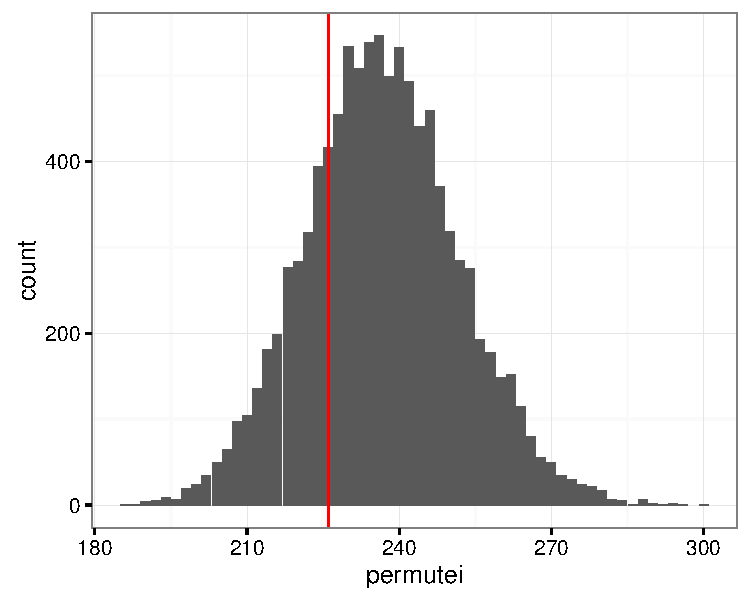
\includegraphics[width=\maxwidth]{figure/t12b-1} 

\end{knitrout}





\begin{knitrout}
\definecolor{shadecolor}{rgb}{0.969, 0.969, 0.969}\color{fgcolor}\begin{kframe}
\begin{alltt}
\hlcom{#checking exchangeability for y2 total excess minutes}
\hlcom{#or like this? instead permute obs from trial 1 and trial 2?}
\hlcom{#obsy2 <- sum(trial1$totalexcess-trial2$totalexcess)#cor(trial1$totalexcess,trial2$totalexcess)}
\hlstd{obsy2} \hlkwb{<-} \hlkwd{coef}\hlstd{(}\hlkwd{lm}\hlstd{(trial1}\hlopt{$}\hlstd{totalexcess}\hlopt{~}\hlstd{trial2}\hlopt{$}\hlstd{totalexcess))[}\hlnum{2}\hlstd{]}
\hlstd{nsim} \hlkwb{<-} \hlnum{10000}
\hlstd{permutey2} \hlkwb{<-} \hlkwd{rep}\hlstd{(}\hlnum{0}\hlstd{,nsim)}
\hlstd{nboutmaty2} \hlkwb{<-} \hlkwd{cbind}\hlstd{(trial1}\hlopt{$}\hlstd{totalexcess,trial2}\hlopt{$}\hlstd{totalexcess)}
\hlstd{newmaty2} \hlkwb{<-} \hlkwd{matrix}\hlstd{(}\hlnum{0}\hlstd{,}\hlkwc{nrow}\hlstd{=}\hlkwd{nrow}\hlstd{(nboutmaty2),}\hlkwc{ncol}\hlstd{=}\hlkwd{ncol}\hlstd{(nboutmaty2))}
\hlkwa{for}\hlstd{(i} \hlkwa{in} \hlnum{1}\hlopt{:}\hlstd{nsim)\{}
  \hlkwa{for}\hlstd{(j} \hlkwa{in} \hlnum{1}\hlopt{:}\hlkwd{nrow}\hlstd{(nboutmaty2))\{}
    \hlstd{s} \hlkwb{<-} \hlkwd{sample}\hlstd{(}\hlnum{1}\hlopt{:}\hlnum{2}\hlstd{,}\hlnum{2}\hlstd{)}
    \hlstd{newmaty2[j,s[}\hlnum{1}\hlstd{]]} \hlkwb{<-} \hlstd{nboutmaty2[j,}\hlnum{1}\hlstd{]}
    \hlstd{newmaty2[j,s[}\hlnum{2}\hlstd{]]} \hlkwb{<-} \hlstd{nboutmaty2[j,}\hlnum{2}\hlstd{]}
  \hlstd{\}}

  \hlcom{#permutey2[i] <- sum(newmaty2[,1]-newmaty2[,2])#cor(newmaty2)[1,2]}
  \hlstd{permutey2[i]} \hlkwb{<-} \hlkwd{coef}\hlstd{(}\hlkwd{lm}\hlstd{(newmaty2[,}\hlnum{1}\hlstd{]}\hlopt{~}\hlstd{newmaty2[,}\hlnum{2}\hlstd{]))[}\hlnum{2}\hlstd{]}\hlcom{#cor(newmaty2)[1,2]}

\hlstd{\}}

\hlkwd{qplot}\hlstd{(}\hlkwc{x}\hlstd{=permutey2)} \hlopt{+} \hlkwd{geom_vline}\hlstd{(}\hlkwc{xintercept}\hlstd{=obsy2,}\hlkwc{col}\hlstd{=}\hlstr{"red"}\hlstd{)} \hlopt{+} \hlkwd{theme_bw}\hlstd{()}
\end{alltt}


{\ttfamily\noindent\itshape\color{messagecolor}{\#\# `stat\_bin()` using `bins = 30`. Pick better value with `binwidth`.}}\end{kframe}
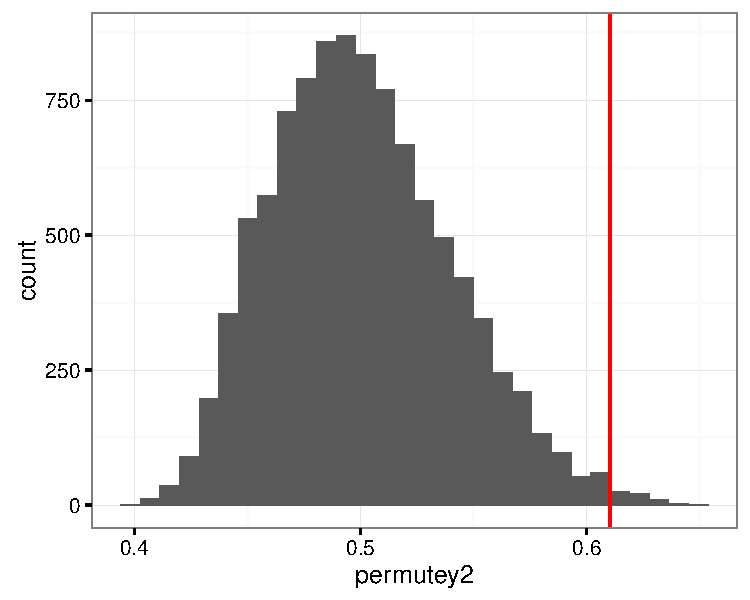
\includegraphics[width=\maxwidth]{figure/t14-1} 

\end{knitrout}

\begin{knitrout}
\definecolor{shadecolor}{rgb}{0.969, 0.969, 0.969}\color{fgcolor}\begin{kframe}


{\ttfamily\noindent\itshape\color{messagecolor}{\#\# `stat\_bin()` using `bins = 30`. Pick better value with `binwidth`.}}\end{kframe}
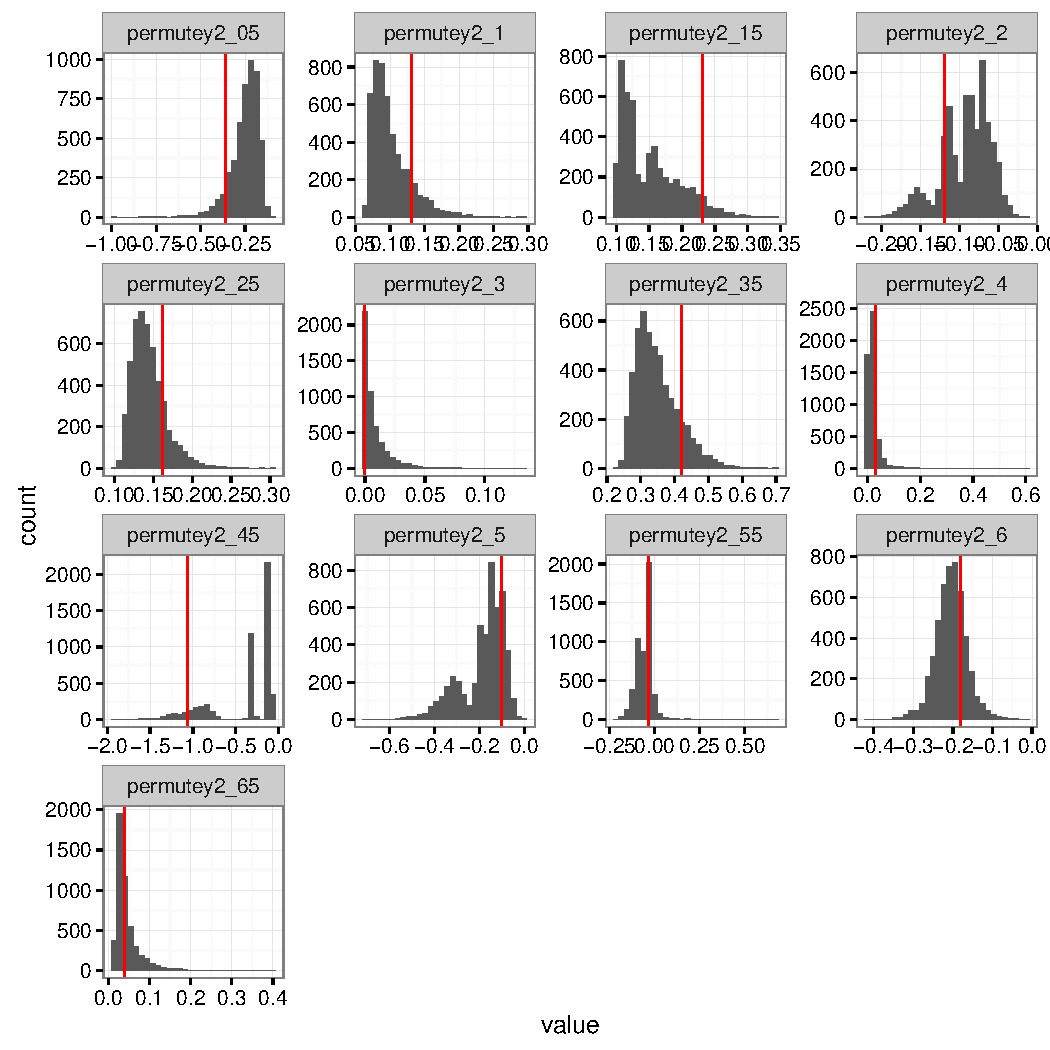
\includegraphics[width=\maxwidth]{figure/t15-1} 
\begin{kframe}\begin{verbatim}
##  [1] 0.0800 0.8566 0.9380 0.1660 0.8268 0.1682 0.8546 0.8466 0.0844 0.8180
## [11] 0.7664 0.7506 0.5918
\end{verbatim}
\end{kframe}
\end{knitrout}

\end{document}
